
\subsection{Problem Formulation and Overall Framework}
\label{sec:method-overview}

Predicting the surface pressure of transonic wings with limited high-fidelity data requires exploiting transferable sectional aerodynamic information while accounting for three-dimensional flow effects. To address this challenge, a hierarchical knowledge-transfer method is developed to separately represent the baseline sectional pressure response and localized pressure corrections near the wing root and tip. These knowledge components are transferred to the target wing to construct a three-dimensional pressure prior, while a residual model trained on limited target-domain CFD data learns the remaining pressure discrepancy.

For a wing with spanwise-varying airfoil geometry and planform parameters, let $\eta=z/(b/2)$ denote the normalized spanwise coordinate and $\xi=x/c(\eta)$ the local chord-normalized coordinate. The predicted surface pressure coefficient is expressed as
\begin{equation}
    \widehat{C}_{p,s}^{3D}(\eta,\xi)
    = C_{p,s}^{\mathrm{prior}}(\eta,\xi)
    + \widehat{R}_{p,s}^{\mathrm{tar}}(\eta,\xi),
    \qquad s\in\{u,l\},
    \label{eq:hierarchical-pressure-decomposition}
\end{equation}
where $u$ and $l$ denote the upper and lower surfaces, respectively. The pressure prior $C_{p,s}^{\mathrm{prior}}$ combines the baseline sectional response with regional finite-span corrections, whereas $\widehat{R}_{p,s}^{\mathrm{tar}}$ represents the residual pressure discrepancy learned from target-domain data.

The overall framework is illustrated in Fig.~\ref{fig:hierarchical-framework}. A sectional baseline model is pretrained using infinite-span swept-wing data, while separate root and tip correction models are developed from paired finite- and infinite-span pressure differences. For a given target-wing geometry and flow condition, the pretrained knowledge models are combined through sectionwise mapping, spanwise gating, and amplitude calibration to construct the pressure prior. With the knowledge models frozen, a target-domain residual network incorporates geometric and flow information, the pressure prior, and pretrained sectional features to predict the remaining pressure correction. High-fidelity target-domain CFD data provide supervision during training, whereas inference requires only the target geometry and flow conditions. The resulting surface-pressure predictions are further used as inputs to separately trained aerodynamic-coefficient regression models.

\begin{figure*}[t]
    \centering
    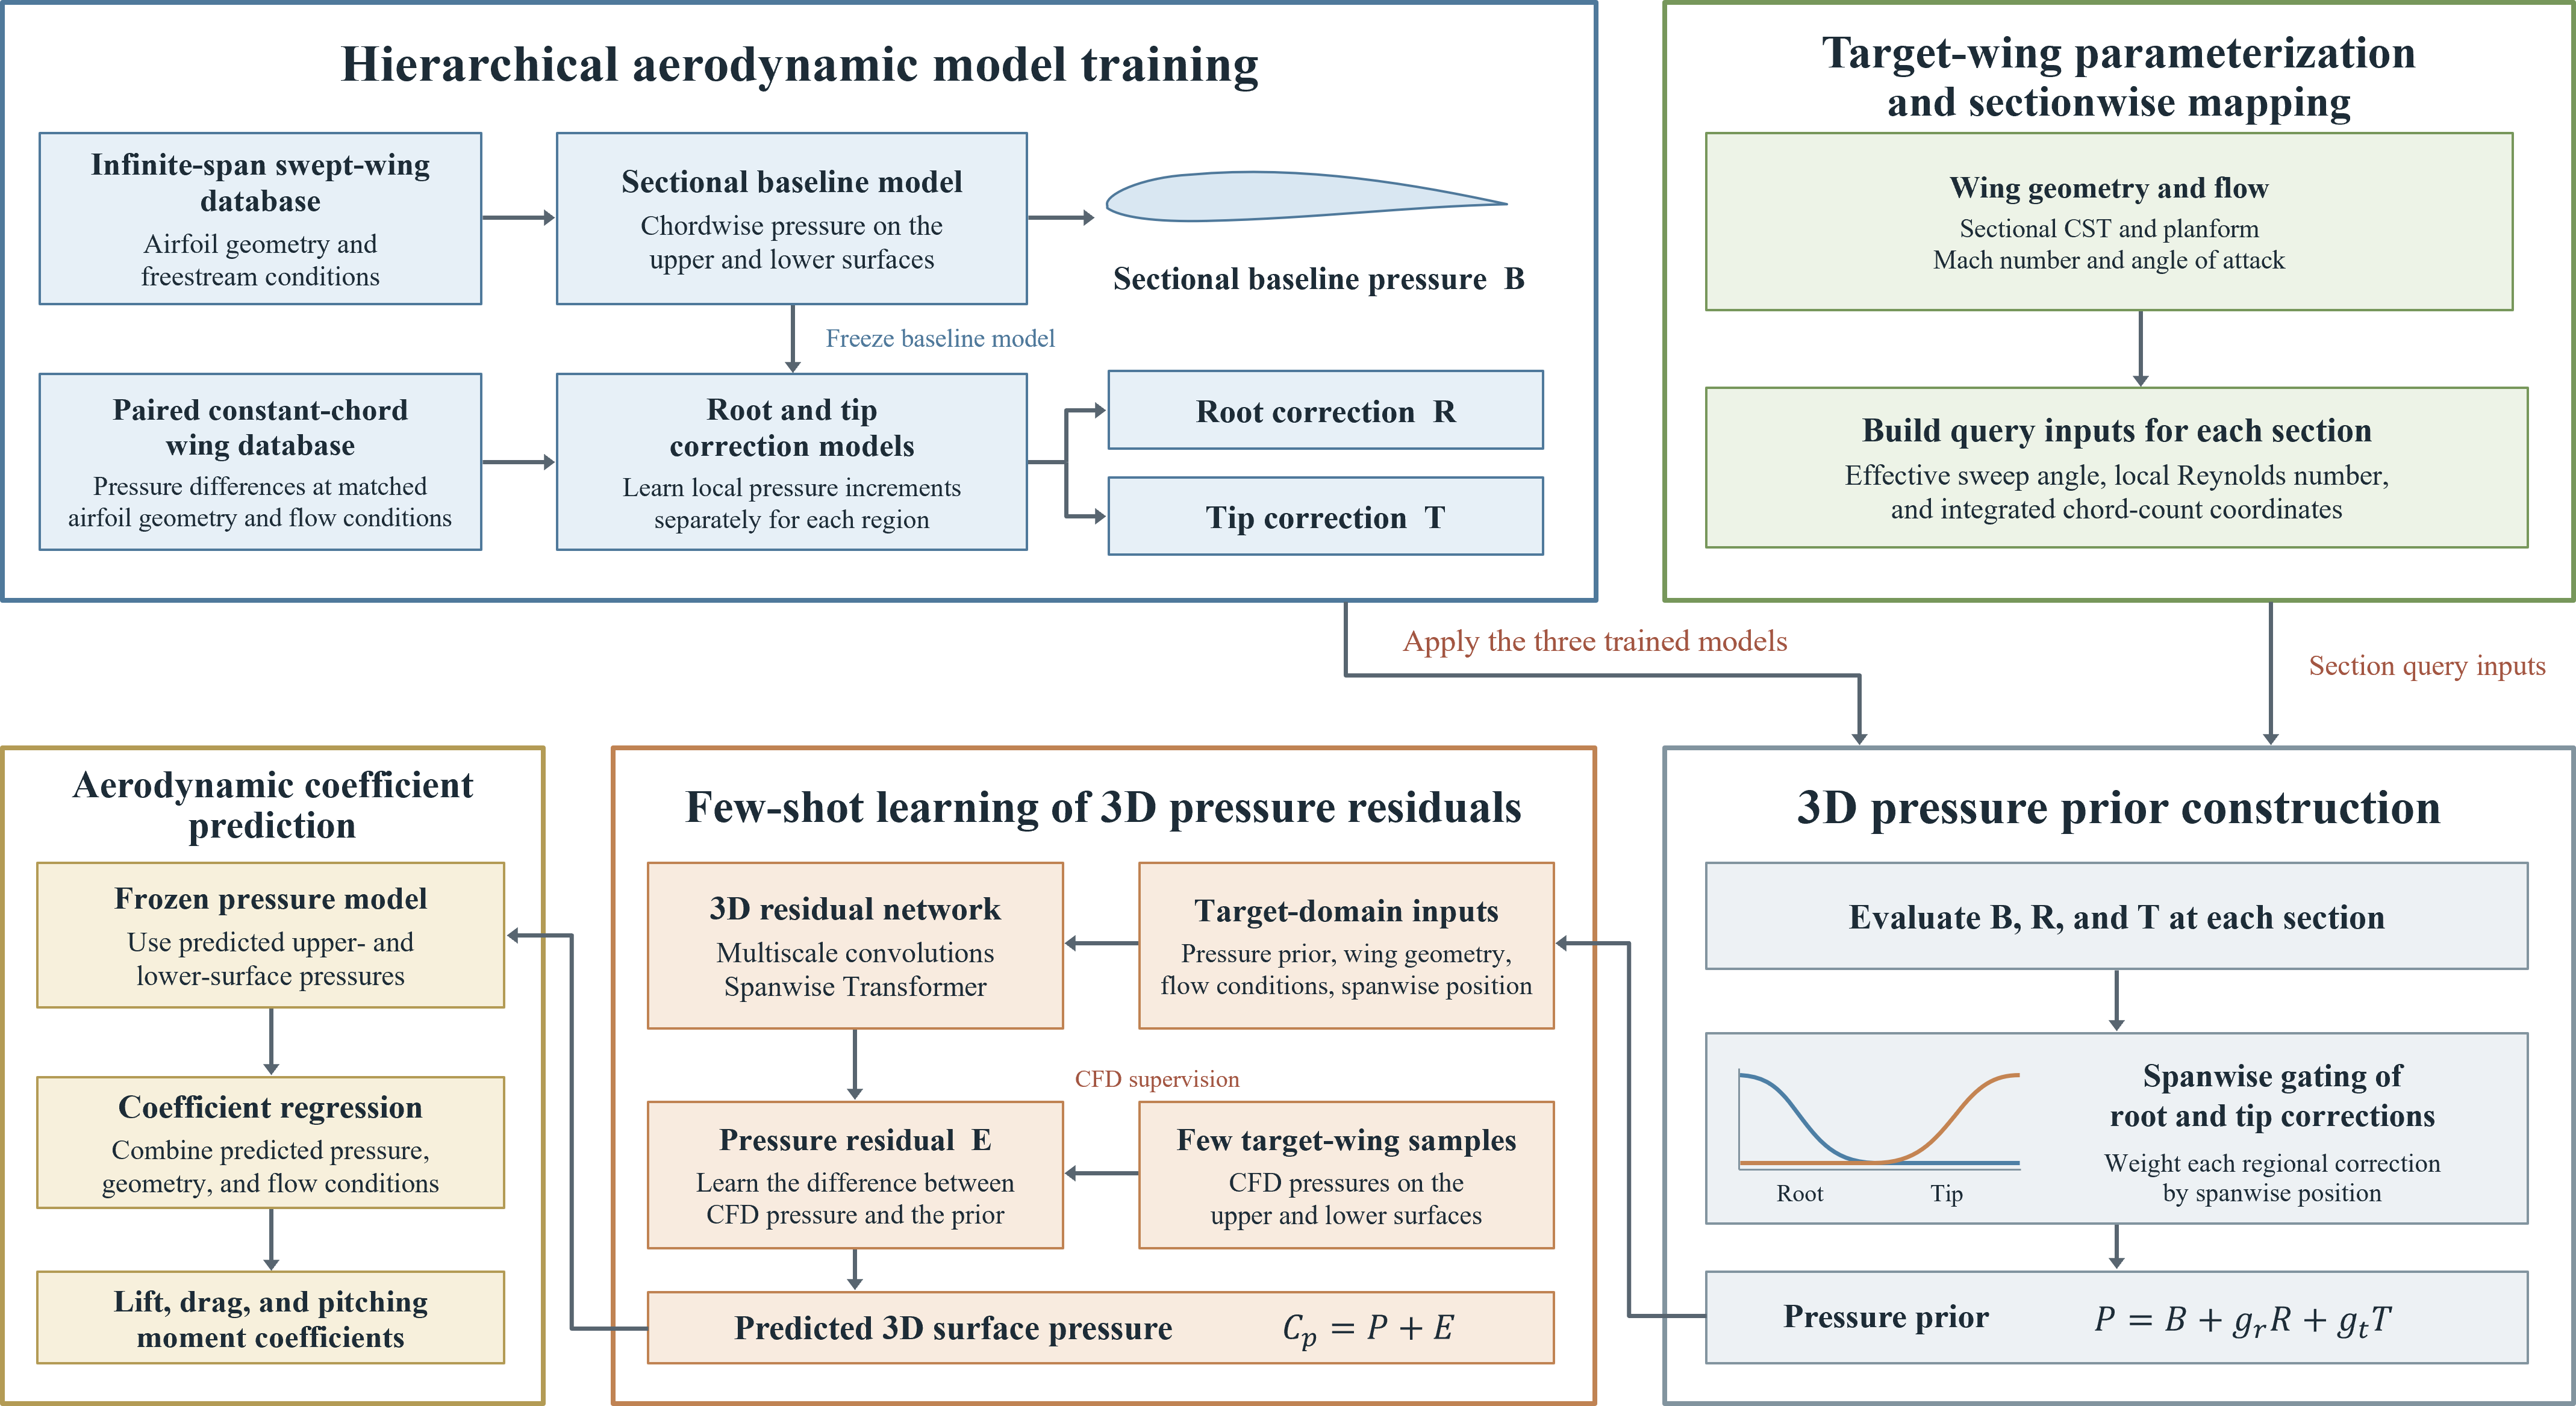
\includegraphics[width=\textwidth]{III_Knowledge_Transfer/figures/III_A_Fig08/III_A_Fig08_hierarchical_framework_v2.png}
    \caption{Hierarchical aerodynamic knowledge-transfer framework for wing surface-pressure prediction and aerodynamic-coefficient regression.}
    \label{fig:hierarchical-framework}
\end{figure*}
